\documentclass[a4]{beamer}
\usepackage{amssymb}
\usepackage{graphicx}
\usepackage{subfigure}
\usepackage{newlfont}
\usepackage{amsmath,amsthm,amsfonts}
%\usepackage{beamerthemesplit}
\usepackage{pgf,pgfarrows,pgfnodes,pgfautomata,pgfheaps,pgfshade}
\usepackage{mathptmx}  % Font Family
\usepackage{helvet}   % Font Family
\usepackage{color}

\mode<presentation> {
 \usetheme{Frankfurt} % was Frankfurt
 \useinnertheme{rounded}
 \useoutertheme{infolines}
 \usefonttheme{serif}
 %\usecolortheme{wolverine}
% \usecolortheme{rose}
\usefonttheme{structurebold}
}

\setbeamercovered{dynamic}

\title[MA4413]{Statistics for Computing \\ {\normalsize MA4413 Lecture 4B}}
\author[Kevin O'Brien]{Kevin O'Brien \\ {\scriptsize Kevin.obrien@ul.ie}}
\date{Autumn Semester 2012}
\institute[Maths \& Stats]{Dept. of Mathematics \& Statistics, \\ University \textit{of} Limerick}

\renewcommand{\arraystretch}{1.5}

\begin{document}
%----------------------------------------------------%
\begin{frame}
\frametitle{Central Limit Theorem}

\begin{itemize}

\item Before we can begin computing confidence intervals, we must introduce the \textbf{\emph{Central Limit Theorem}}.

\item Suppose random sample of size $n$ are drawn from any distribution, with the distribution having a mean of $\mu$ (equivalently $E(X)$) and variance of $\sigma^2$ (i.e. standard deviation of $\sigma$).

\item Also suppose that the sample size is large ( i.e. $n > 30$ ).

\item The sample means tend to form a normal distribution with mean $\mu$ and standard deviation $ { \sigma \over \sqrt{n} }$

\item We call the standard deviation of the sample means the \textbf{\emph{standard error}}
\item Standard error is commonly denoted as $S.E.$
\end{itemize}
\end{frame}

%----------------------------------------------------%
\begin{frame}
\frametitle{Central Limit Theorem}

\begin{itemize}

\item Recall from earlier lectures, an experiment was carried out where the sum of 100 throws of a die were recorded.

\item The underlying distribution of the die values is not normally distributed. \\(Actually discrete uniform between 1 and 6.)

\item Nonetheless the distribution of the sum of 100 throws was normally distributed. Necessarily the distribution of the average score for 100 throws is normally distributed.

\end{itemize}
\end{frame}

\frame{
\frametitle{Distribution of means}

\begin{center}
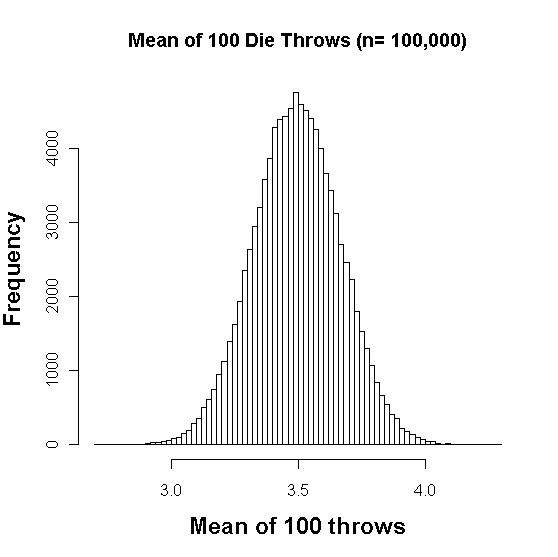
\includegraphics[scale=0.4]{images/6Bhist}
\end{center}

}
%----------------------------------------------------%
\begin{frame}
\frametitle{Exercise}
From previous lecture, we know the following properties of the dice distribution. \\(Remark: In this case we know the variance, but that is not always the case.)
\begin{itemize}
\item Mean (Expected Value) $E(X) = \mu = 3.5$
\item Variance $V(X) = \sigma^2 = 2.9166$
\item Standard deviation $= \sigma = 1.707$
\end{itemize}

Compute the standard error $S.E.(\bar{x})$ for the mean value $\bar{x}$ of die values:
\begin{itemize}
\item when the die is thrown 25 times
\item when the die is thrown 225 times.
\end{itemize}
\end{frame}

%----------------------------------------------------%
\begin{frame}
\frametitle{Exercise}
\begin{itemize}
\item When the die is thrown 25 times n = 25
\item Therefore the standard error is
\[ {\sigma \over \sqrt{n}}  = {1.707 \over \sqrt{25}} = {1.707 \over 5} = 0.3415. \]
\item When the die is thrown 225 times: n = 225
\item Therefore the standard error is
\[ {\sigma \over \sqrt{n}}  = {1.707 \over \sqrt{225}} = {1.707 \over 15} = 0.1138. \]

\end{itemize}
\end{frame}
\frame{
\frametitle{Distribution of means}

\begin{center}
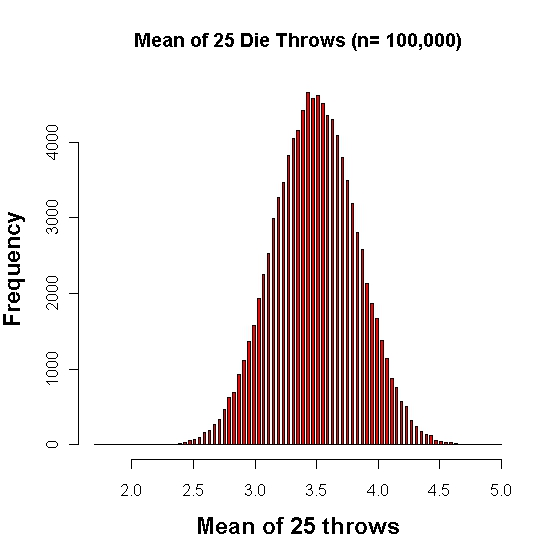
\includegraphics[scale=0.4]{images/6Bhist2}
\end{center}

}

\frame{
\frametitle{Distribution of means}

\begin{center}
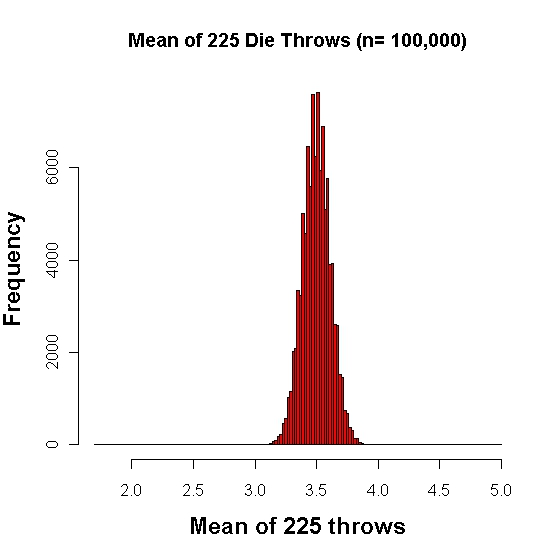
\includegraphics[scale=0.4]{images/6Bhist3}
\end{center}

}

%----------------------------------------------------%
\begin{frame}
\frametitle{Exercise}
\begin{itemize}
\item Compare the two histograms on the previous slides. These horizontal range of value is the same for both histograms.

\item We can see that with a larger sample size ($n=225$), the distribution of sample means are clustered closely around the 3.5 mark, and have much less dispersion than distribution of sample means with a sample size $n=25$.

\end{itemize}
\end{frame}
\begin{frame}
\frametitle{Confidence Intervals (Revision) }

\begin{itemize}
\item The $95\%$ confidence interval is a range of values which contain the true population parameter (i.e. mean, proportion etc) with a probability of $95\%$.
\item We can expect that a $95\%$ confidence interval will not include the true parameter values $5\%$ of the time.
\item A confidence level of $95\%$ is commonly used for computing confidence interval, but we could also have confidence levels of $90\%$,$99\%$ and $99.9\%$.
\end{itemize}

\end{frame}

%-----------------------------------------------------------%


\begin{frame}
\frametitle{Confidence Level}

\begin{itemize}
\item A confidence level for an interval is denoted to $1-\alpha$ (in percentages: $100(1-\alpha)\%$) for some value $\alpha$.
\item A confidence level of $95\%$ corresponds to $\alpha = 0.05$.
\item $100(1-\alpha)\%$ = $100(1-0.05)\%$  = $100(0.95)\%$ = $95\%$
\item For a confidence level of $99\%$, $\alpha = 0.01$.
\item Knowing the correct value for $\alpha$ is important when determining quantiles.
\end{itemize}

\end{frame}


%-----------------------------------------------------------%
\begin{frame}
\frametitle{The Central Limit Theorem}
\begin{itemize}
\item This theorem states that as sample size $n$ is increased, the sampling distribution of the mean (and for other sample statistics as well) approaches the normal distribution in form, regardless of the form of the population distribution from
which the sample was taken.

\item For practical purposes, the sampling distribution of the mean can be assumed to be
approximately normally distributed, even for the most non-normal populations or processes, whenever the
sample size is $n > 30$.

\item (For populations that are only somewhat non-normal, even a smaller sample size will
suffice. A variation of the normal distribution can be used for such circumstances.)
\end{itemize}


\end{frame}
%-----------------------------------------------------------%


\begin{frame}
\frametitle{Computing Confidence Intervals}
Confidence limits are the lower and upper boundaries / values of a confidence interval, that is, the values which define the range of a confidence interval. The general structure of a confidence interval is as follows:

\[ \mbox{Point Estimate}  \pm \left[ \mbox{Quantile} \times \mbox{Standard Error} \right] \]


\begin{itemize}
\item Point Estimate: estimate for population parameter of interest, i.e. sample mean, sample proportion.
\item Quantile: a value from a probability distribution that scales the intervals according to the specified confidence level.
\item Standard Error: measures the dispersion of the sampling distribution for a given sample size $n$.
\end{itemize}
\end{frame}


%-----------------------------------------------------------%

\begin{frame}
\frametitle{Point Estimates (1) }

\begin{itemize}
\item Point estimates are generally straightforward calculations.
\item Sometimes they will even be stated directly in the questions.
\item When considering the population mean $\mu$, the appropriate point estimate is the sample mean $\bar{x}$.
\item When considering the population proportion $\pi$, the appropriate point estimate is the sample proportion $\hat{p}$.
\end{itemize}

\end{frame}
%------------------------------------------------------------------------------%
\frame{
\frametitle{Point Estimates (2) }

Sample percentage

\[
\hat{p} = \frac{x}{n} \times 100\%
\]

\begin{itemize}
\item $\hat{p}$ - sample proportion.
\item $x$  - number of ``successes".
\item $n$  - the sample size.
\end{itemize}

}
%------------------------------------------------------------------------------%
\frame{
\frametitle{Point Estimates (3)}

Of a sample of 160 computer programmers, 56 reported than Python was their primary programming language.

Let $\pi$ be the proportion of all programmers who regard Python as their programming language. What is the point estimate for $\pi$?

\[
\hat{p} = \frac{x}{n} \times 100\%  = {56 \over 160} = 35\%
\]



}
\end{document}

